\section{Preparação dos modelos}
\label{sec:metodos-preparacao-modelos}

% Uma vez que temos um \textit{dataset} com atributos fonológicos processados, agora podemos prosseguir com a preparação das features e dos modelos para reconhecimentos dos sinais utilizando a abordagem proposta.


% Experimento
%   Preparação das features (asl-phono -> palavras)
%       Transformação das sequências no dataset: frames -> palavras
%       Justificativa??
%   Preparação dos modelos (Transformer, LSTM, GRU, etc) -- por modelo
%       Arquitetura + Parâmetros
%       lr scheduler, optimizer, loss function
%       Busca de parâmetros (dimensionar os modelos/parâmetros)

% %FIXME: [cz] essa parte ficaria na metodologia se vc tirar a os datasets para uma nova secao

% SELEÇÃO DOS MODELOS -------------------------------------------

Tomando como referência a discussão introduzida na \autoref{sec:am-ap}, serão adotados nos experimentos deste trabalho três das principais arquiteturas utilizadas em tarefas de \acrfull{nlp}: o \textit{Encoder-Decoder} em uma versão com \acrfull{lstm} e outra com \acrfull{gru}, e também o \textit{Transformer}.

% Os parâmetros para treinamento dos modelos foram selecionados com base na discussão apresentada por \citeonline{goodfellow-2016-deep-learning}, a qual aborda de forma prática temas como definição de métricas, modelos de base, otimização de parâmetros, entre outros para tal finalidade.

Para estabelecer os parâmetros dessas arquiteturas, as estratégias de otimização e de treinamento, bem como as métricas utilizadas nos experimentos, foram consideradas as discussões apresentadas por \citeonline{goodfellow-2016-deep-learning} e pela \autoref{sec:am}.

Dessa forma, o algoritmo de otimização dos modelos será definido como o \acrfull{sgd} com \textit{momentum} de 0,9 \cite{robbins-2007-stochastic}. Ele será combinado a uma estratégia de redução da taxa de aprendizagem por um fator de 0,2 sempre que o valor do erro médio calculado atingir um platô por 5 épocas seguidas.

A função objetivo (ou função de perda), por sua vez, será a \acrfull{cel} \cite{mitchell-1997-ml}, que é apresentada na \autoref{eqn:cross-entropy-loss}. Nela, \(p\) representa as probabilidades ou pontuações estimadas pelo modelo para as amostras e \(y\) corresponde ao valor correto esperado para essas estimativas:

\begin{equation}
    \label{eqn:cross-entropy-loss}
    L_{\log}(y, p) = -(y \log (p) + (1 - y) \log (1 - p))
\end{equation}


Os dados serão particionados numa proporção de 15\% para o subconjunto de validação, 15\% para o de testes e o restante para o subconjunto treinamento. Os \textit{batches} (ou lotes), por sua vez, possuirão tamanho de 50 amostras.

% Dessa forma, utilizamos como algoritmo de otimização o \acrfull{sgd} com \textit{momentum} de 0,9. Ele foi combinado com uma estratégia de redução da taxa de aprendizagem por um fator de 0,2 sempre que o valor da perda calculada sobre os dados de validação atinge um platô por 5 épocas seguidas. A função de perda utilizada, por sua vez, foi a \textit{Cross-Entropy Loss} (ou Perda de Entropia Cruzada). Além disso, adotamos \textit{batches} com tamanho de 50 amostras e particionamos o \textit{dataset} numa proporção de 15\% para validação, 15\% para testes e o restante para treinamento dos modelos.


% % Parâmetros otimizados para Encoder-Decoder (LSTM):
% \begin{figure}[ht!]
%     \centering
%     \caption{\textmd{Parâmetros otimizados para o \textit{Encoder-Decoder} com \acrshort{lstm}}}
%     \borda[\textwidth]{
%         \subcaptionbox{Taxa de aprendizagem \label{subfig:otim-encdec-lstm-lr}}{
%             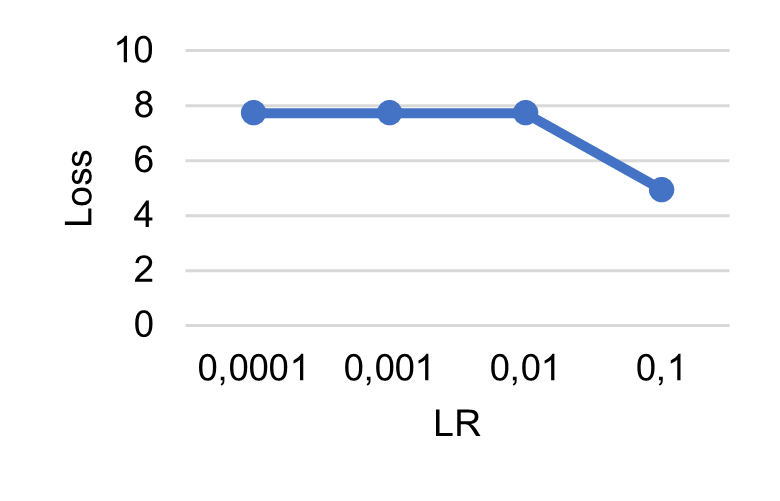
\includegraphics[width=5.0cm]{capitulos/metodos/imagens/otim_encdec_lstm_lr}
%         }%
%         % \hfill
%         \subcaptionbox{Dropout \label{subfig:otim-encdec-lstm-dropout}}{
%             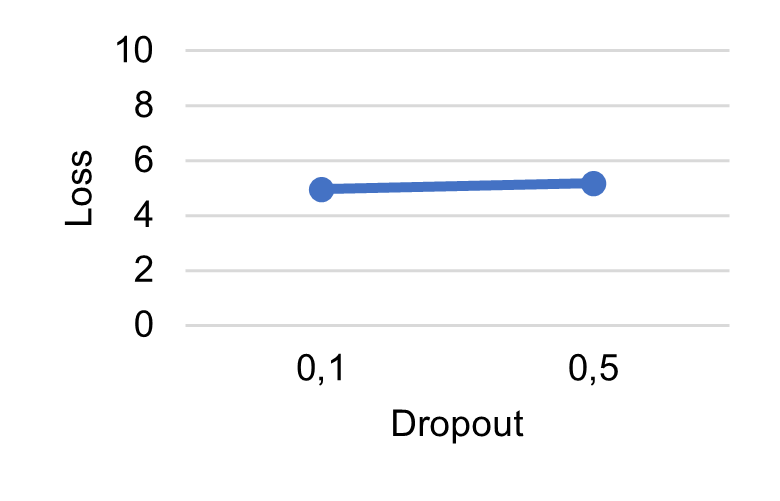
\includegraphics[width=5.0cm]{capitulos/metodos/imagens/otim_encdec_lstm_dropout}
%         }%
%         % \hfill
%         \subcaptionbox{Nº de camadas \label{subfig:otim-encdec-lstm-layers}}{
%             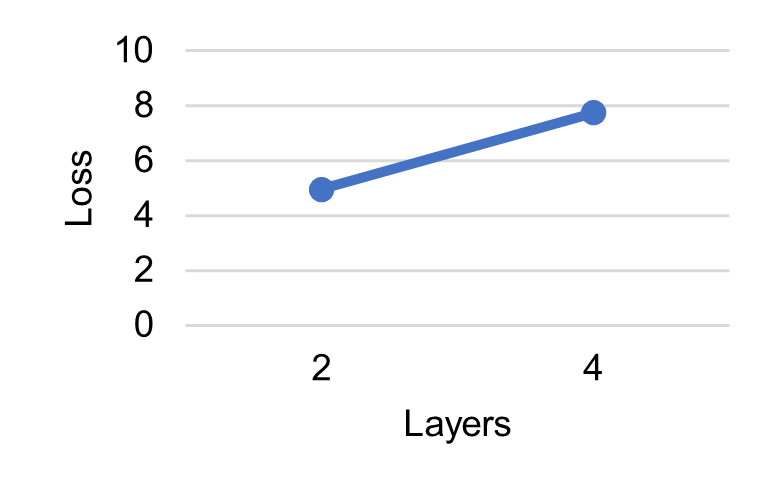
\includegraphics[width=5.0cm]{capitulos/metodos/imagens/otim_encdec_lstm_layers}
%         }%
%         \hfill
%         \subcaptionbox{Tamanho camadas ocultas \label{subfig:otim-encdec-lstm-hidden}}{
%             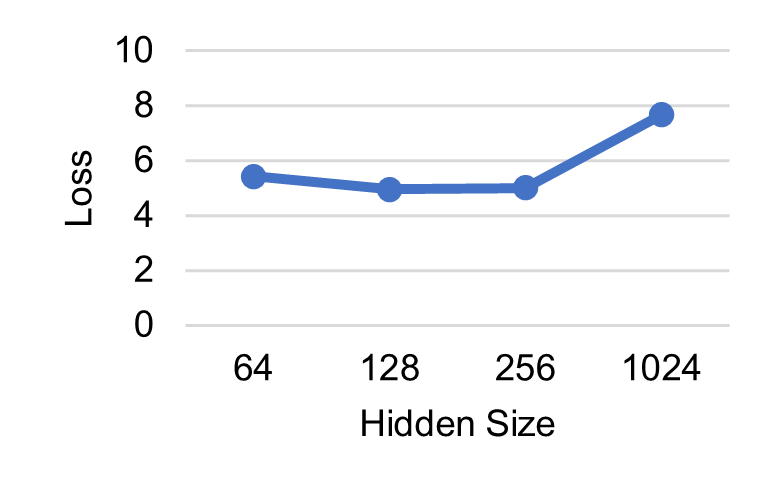
\includegraphics[width=5.0cm]{capitulos/metodos/imagens/otim_encdec_lstm_hidden_size}
%         }%
%         % \hfill
%         \subcaptionbox{Tamanho embeddings \label{subfig:otim-encdec-lstm-emb}}{
%             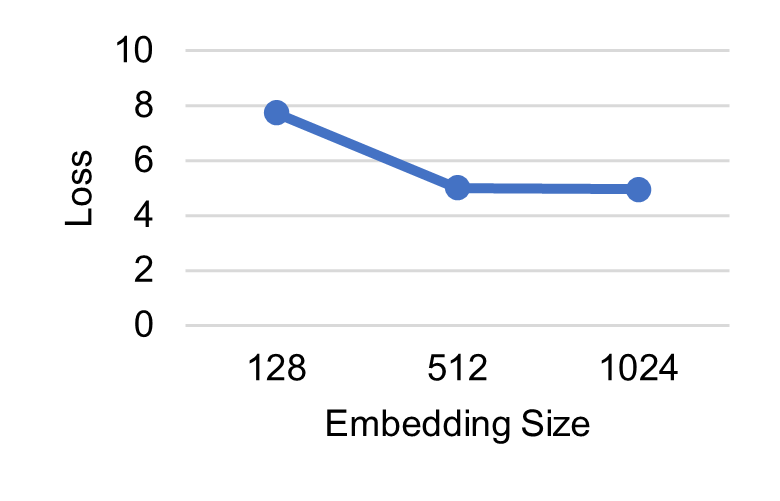
\includegraphics[width=5.0cm]{capitulos/metodos/imagens/otim_encdec_lstm_emb_size}
%         }%
%     }
%     \nomefonte{}
%     \label{fig:otim-encdec-lstm}
% \end{figure}


A seleção dos hiperparâmetros dos modelos foi realizada utilizando-se o algoritmo \textit{Grid Search} (ou busca em grade) com validação cruzada de 5 \textit{folds}. O conjunto de valores de hiperparâmetros utilizados na busca estão apresentados na \autoref{tab:otim-params} e as combinações que melhor reduziram o erro médio para cada modelo foram as seguintes:

% Please add the following required packages to your document preamble:
% \usepackage{multirow}
% \usepackage{graphicx}
% \usepackage[table,xcdraw]{xcolor}
% If you use beamer only pass "xcolor=table" option, i.e. \documentclass[xcolor=table]{beamer}
\begin{table}[]
    \centering
    \caption{Hiperparâmetros otimizados para o \textit{Encoder-Decoder} (\acrshort{lstm}), \textit{Encoder-Decoder} (\acrshort{gru}) e o \textit{Transformer} com os respectivos erros médios calculados (\acrfull{cel})}
    \label{tab:otim-params}
    \resizebox{0.95\textwidth}{!}{%
        \begin{tabular}{lr|rrr}
            \hline
            \rowcolor[HTML]{EFEFEF}
            \multicolumn{2}{l|}{\cellcolor[HTML]{EFEFEF}}                                                             & \multicolumn{3}{c}{\cellcolor[HTML]{EFEFEF}Erro médio (\acrshort{cel})}                                                                                                                                                                                                     \\ \cline{3-5}
            \rowcolor[HTML]{EFEFEF}
            \multicolumn{2}{l|}{\multirow{-2}{*}{\cellcolor[HTML]{EFEFEF}Hiperparâmetro}}                                  & \multicolumn{1}{c|}{\cellcolor[HTML]{EFEFEF}\textbf{Encoder-Decoder (LSTM)}} & \multicolumn{1}{c|}{\cellcolor[HTML]{EFEFEF}\textbf{Encoder-Decoder (GRU)}} & \multicolumn{1}{c}{\cellcolor[HTML]{EFEFEF}\textbf{Transformer}}                                    \\ \hline
            \multicolumn{1}{l|}{}                                                                                     & 0,001                                                                        & \multicolumn{1}{r|}{7,734342}                                               & \multicolumn{1}{r|}{7,263981}                                    & 2,579863                         \\
            \multicolumn{1}{l|}{}                                                                                     & 0,01                                                                         & \multicolumn{1}{r|}{6,000810}                                               & \multicolumn{1}{r|}{\cellcolor[HTML]{FFF5E1}4,253146}            & 0,000009                         \\
            \multicolumn{1}{l|}{\multirow{-3}{*}{Taxa de aprendizagem}}                                               & 0,1                                                                          & \multicolumn{1}{r|}{\cellcolor[HTML]{FFF5E1}4,787887}                       & \multicolumn{1}{r|}{4,313777}                                    & \cellcolor[HTML]{FFF5E1}0,000000 \\ \hline
            \multicolumn{1}{l|}{}                                                                                     & 0,1                                                                          & \multicolumn{1}{r|}{\cellcolor[HTML]{FFF5E1}4,787887}                       & \multicolumn{1}{r|}{\cellcolor[HTML]{FFF5E1}4,253146}            & 0,000005                         \\
            \multicolumn{1}{l|}{\multirow{-2}{*}{Dropout}}                                                            & 0,5                                                                          & \multicolumn{1}{r|}{4,942306}                                               & \multicolumn{1}{r|}{4,336690}                                    & \cellcolor[HTML]{FFF5E1}0,000000 \\ \hline
            \multicolumn{1}{l|}{}                                                                                     & 128                                                                          & \multicolumn{1}{r|}{5,871544}                                               & \multicolumn{1}{r|}{5,102946}                                    & 0,000005                         \\
            \multicolumn{1}{l|}{}                                                                                     & 512                                                                          & \multicolumn{1}{r|}{5,096612}                                               & \multicolumn{1}{r|}{4,509590}                                    & \cellcolor[HTML]{FFF5E1}0,000000 \\
            \multicolumn{1}{l|}{\multirow{-3}{*}{Tamanho embeddings}}                                                 & 1024                                                                         & \multicolumn{1}{r|}{\cellcolor[HTML]{FFF5E1}4,787887}                       & \multicolumn{1}{r|}{\cellcolor[HTML]{FFF5E1}4,253146}            & 0,000000                         \\ \hline
            \multicolumn{1}{l|}{}                                                                                     & 128                                                                          & \multicolumn{1}{r|}{4,926501}                                               & \multicolumn{1}{r|}{4,481058}                                    & 0,000000                         \\
            \multicolumn{1}{l|}{}                                                                                     & 256                                                                          & \multicolumn{1}{r|}{4,822424}                                               & \multicolumn{1}{r|}{4,296523}                                    & 0,000000                         \\
            \multicolumn{1}{l|}{\multirow{-3}{*}{\begin{tabular}[c]{@{}l@{}}Tamanho camadas \\ ocultas\end{tabular}}} & 512                                                                          & \multicolumn{1}{r|}{\cellcolor[HTML]{FFF5E1}4,787887}                       & \multicolumn{1}{r|}{\cellcolor[HTML]{FFF5E1}4,253146}            & \cellcolor[HTML]{FFF5E1}0,000000 \\ \hline
            \multicolumn{1}{l|}{}                                                                                     & 2                                                                            & \multicolumn{1}{r|}{\cellcolor[HTML]{FFF5E1}4,787887}                       & \multicolumn{1}{r|}{\cellcolor[HTML]{FFF5E1}4,253146}            & \cellcolor[HTML]{FFF5E1}0,000000 \\
            \multicolumn{1}{l|}{}                                                                                     & 4                                                                            & \multicolumn{1}{r|}{7,734434}                                               & \multicolumn{1}{r|}{5,433316}                                    & 0,000391                         \\
            \multicolumn{1}{l|}{\multirow{-3}{*}{Nº de camadas}}                                                      & 6                                                                            & \multicolumn{1}{r|}{7,734549}                                               & \multicolumn{1}{r|}{7,178291}                                    & 0,016886                         \\ \hline
            \multicolumn{1}{l|}{}                                                                                     & 4                                                                            & \multicolumn{1}{r|}{}                                                       & \multicolumn{1}{r|}{}                                            & 0,000000                         \\
            \multicolumn{1}{l|}{\multirow{-2}{*}{Nº de cabeças}}                                                      & 8                                                                            & \multicolumn{1}{r|}{\multirow{-2}{*}{N/A}}                                  & \multicolumn{1}{r|}{\multirow{-2}{*}{N/A}}                       & \cellcolor[HTML]{FFF5E1}0,000000 \\ \hline
        \end{tabular}%
    }
    \nomefonte{}
\end{table}

\begin{itemize}
    \item \textit{Encoder-Decoder} com \acrshort{lstm}: taxa de aprendizagem de 0,1; \textit{dropout} de 0,1; \textit{embeddings} com dimensão de 1024; camadas ocultas com dimensão de 512; e utilização de 2 camadas de \acrshort{lstm} no \textit{encoder} e no \textit{decoder}.

    \item \textit{Encoder-Decoder} com \acrshort{gru}: taxa de aprendizagem de 0,01; \textit{dropout} de 0,1; \textit{embeddings} com dimensão de 1024; camadas ocultas com dimensão de 512; e utilização de 2 camadas de \acrshort{gru} no \textit{encoder} e no \textit{decoder}.

    \item \textit{Transformer}: taxa de aprendizagem de 0,1; \textit{dropout} de 0,5; \textit{embeddings} com dimensão de 512; camadas ocultas com dimensão de 512; utilização de 2 camadas e de 8 cabeças de \textit{attention}.
\end{itemize}








% % Parâmetros otimizados para Encoder-Decoder (GRU):
% \begin{figure}[ht!]
%     \centering
%     \caption{\textmd{Parâmetros otimizados para o \textit{Encoder-Decoder} com \acrshort{gru}}}
%     \borda[\textwidth]{
%         \subcaptionbox{Taxa de aprendizagem \label{subfig:otim-encdec-gru-lr}}{
%             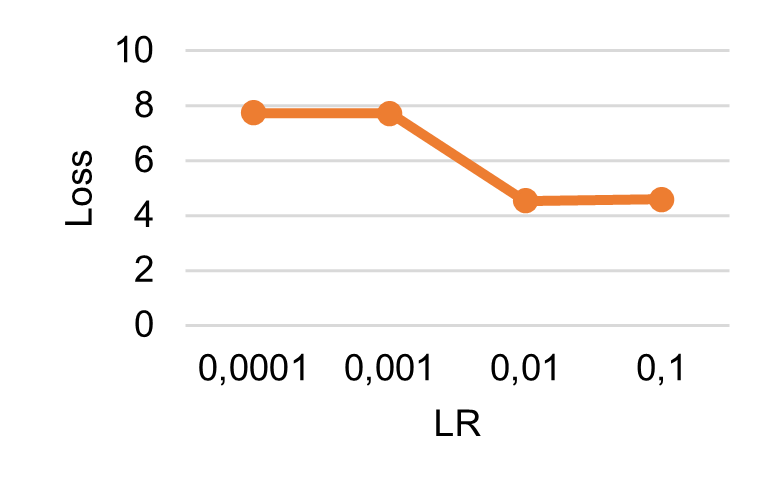
\includegraphics[width=5.0cm]{capitulos/metodos/imagens/otim_encdec_gru_lr}
%         }%
%         % \hfill
%         \subcaptionbox{Dropout \label{subfig:otim-encdec-gru-dropout}}{
%             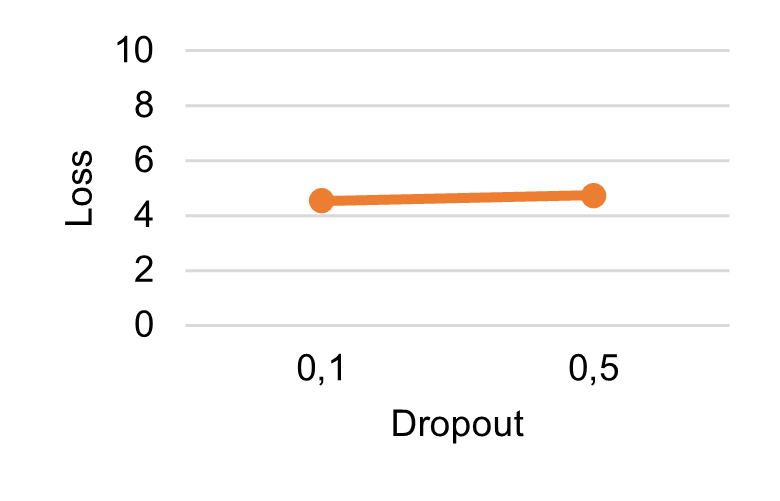
\includegraphics[width=5.0cm]{capitulos/metodos/imagens/otim_encdec_gru_dropout}
%         }%
%         % \hfill
%         \subcaptionbox{Nº de camadas \label{subfig:otim-encdec-gru-layers}}{
%             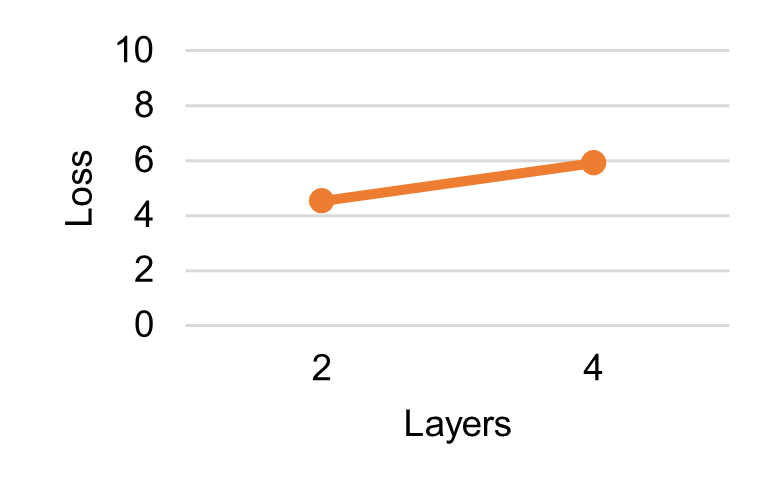
\includegraphics[width=5.0cm]{capitulos/metodos/imagens/otim_encdec_gru_layers}
%         }%
%         \hfill
%         \subcaptionbox{Tamanho camadas ocultas\label{subfig:otim-encdec-gru-hidden}}{
%             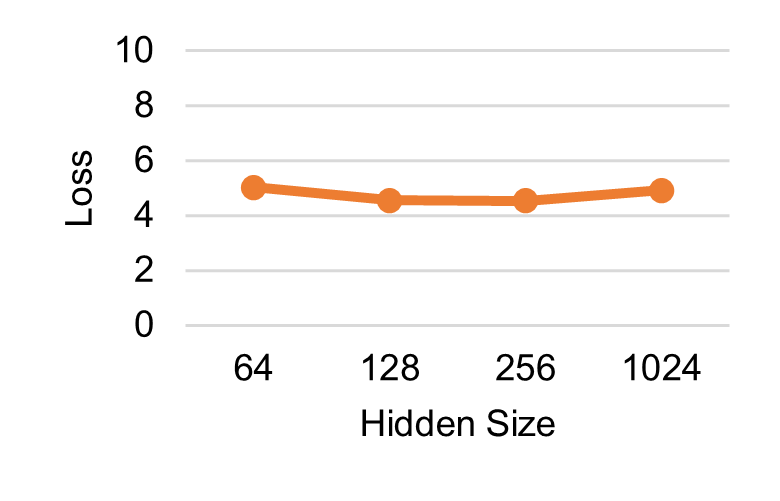
\includegraphics[width=5.0cm]{capitulos/metodos/imagens/otim_encdec_gru_hidden_size}
%         }%
%         % \hfill
%         \subcaptionbox{Tamanho embeddings\label{subfig:otim-encdec-gru-emb}}{
%             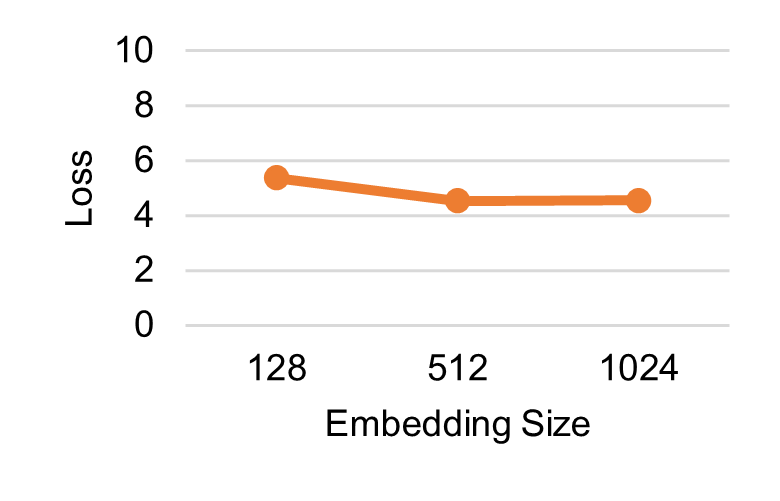
\includegraphics[width=5.0cm]{capitulos/metodos/imagens/otim_encdec_gru_emb_size}
%         }%
%     }
%     \nomefonte{}
%     \label{fig:otim-encdec-gru}
% \end{figure}



% % Parâmetros otimizados para Transformer:
% \begin{figure}[ht!]
%     \centering
%     \caption{\textmd{Parâmetros otimizados para o \textit{Transformer}}}
%     \borda[\textwidth]{
%         \subcaptionbox{Taxa de aprendizagem \label{subfig:otim-transformer-lr}}{
%             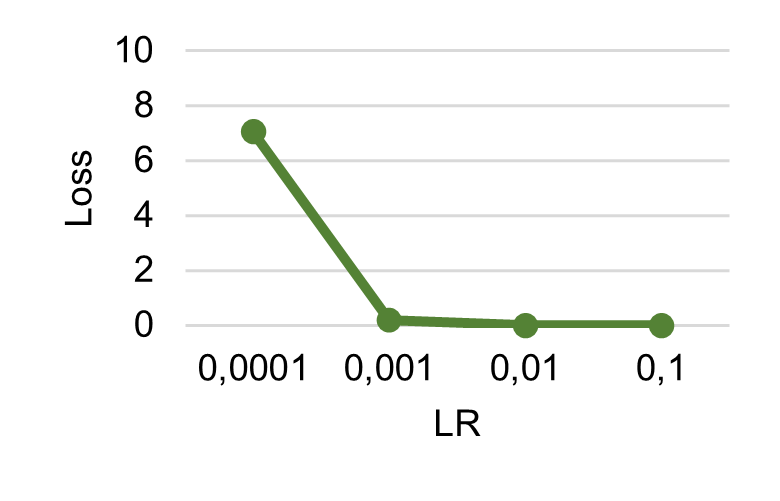
\includegraphics[width=5.0cm]{capitulos/metodos/imagens/otim_transformer_lr}
%         }%
%         % \hfill
%         \subcaptionbox{Dropout \label{subfig:otim-transformer-dropout}}{
%             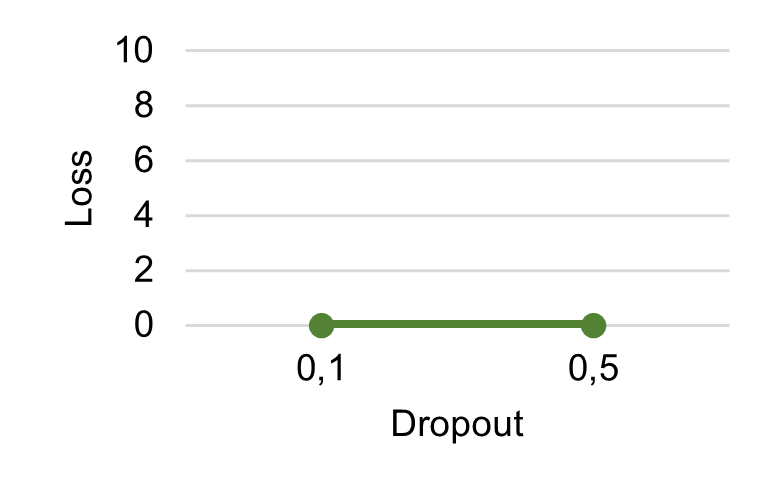
\includegraphics[width=5.0cm]{capitulos/metodos/imagens/otim_transformer_dropout}
%         }%
%         % \hfill
%         \subcaptionbox{Nº de camadas \label{subfig:otim-transformer-layers}}{
%             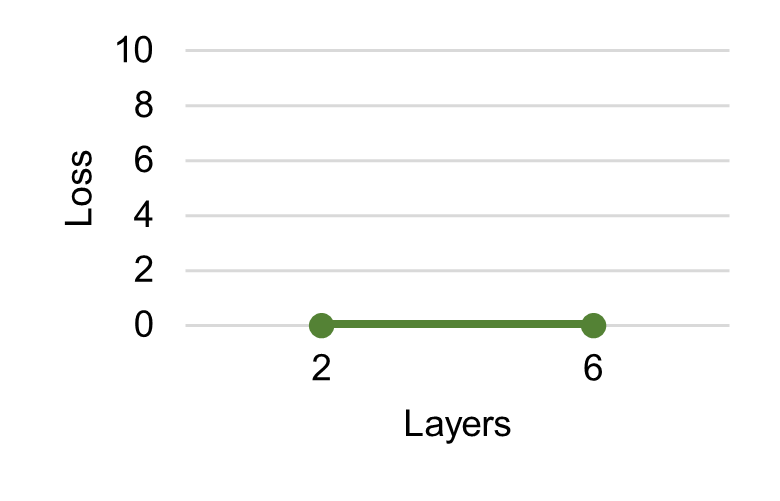
\includegraphics[width=5.0cm]{capitulos/metodos/imagens/otim_transformer_layers}
%         }%
%         \hfill
%         \subcaptionbox{Tamanho camadas ocultas\label{subfig:otim-transformer-hidden}}{
%             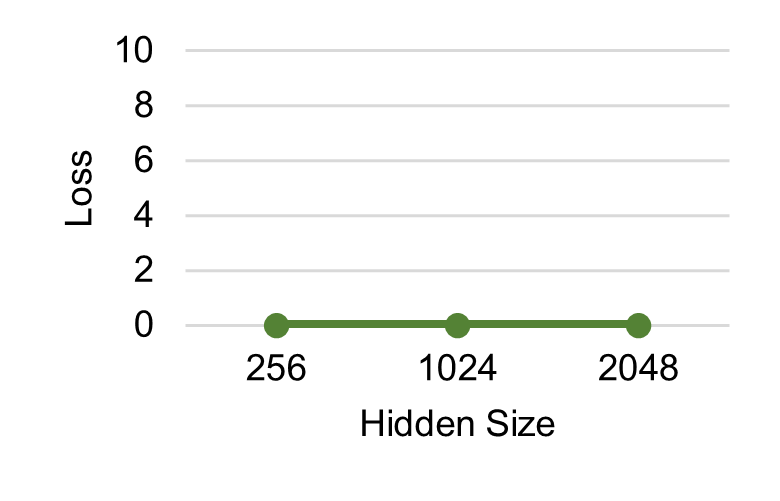
\includegraphics[width=5.0cm]{capitulos/metodos/imagens/otim_transformer_hidden_size}
%         }%
%         % \hfill
%         \subcaptionbox{Tamanho embeddings\label{subfig:otim-transformer-emb}}{
%             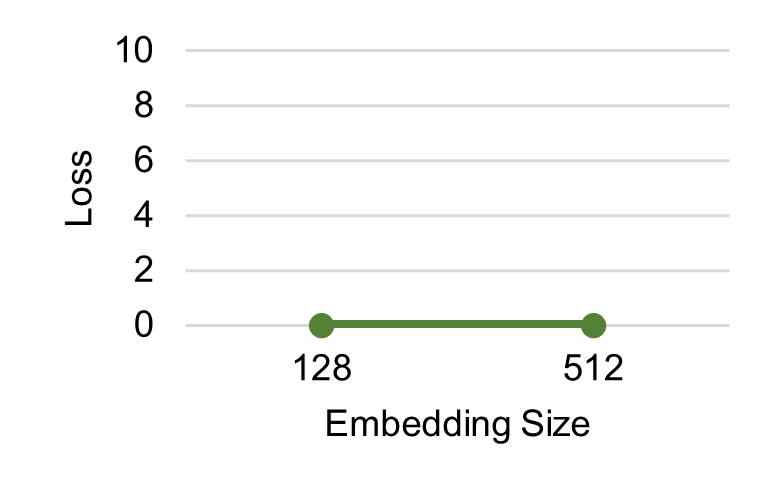
\includegraphics[width=5.0cm]{capitulos/metodos/imagens/otim_transformer_emb_size}
%         }%
%         % \hfill
%         \subcaptionbox{Nº de cabeças\label{subfig:otim-transformer-heads}}{
%             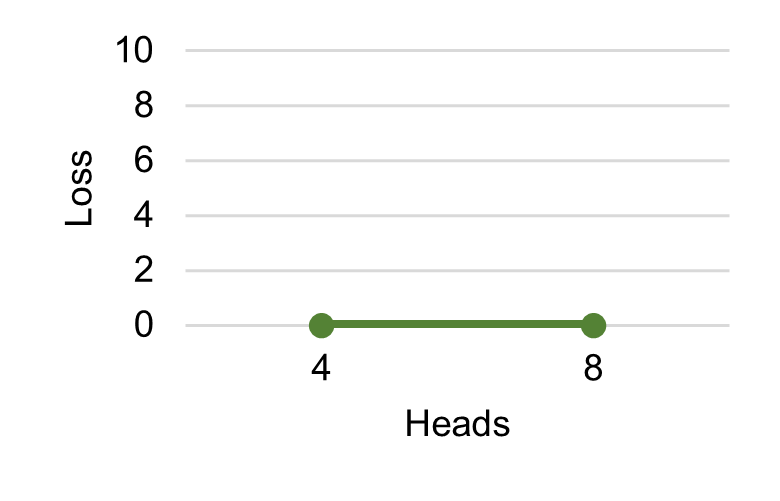
\includegraphics[width=5.0cm]{capitulos/metodos/imagens/otim_transformer_heads}
%         }%
%     }
%     \nomefonte{}
%     \label{fig:otim-transformer}
% \end{figure}






O código-fonte utilizado nos experimentos deste trabalho foi disponibilizado através do endereço indicado abaixo\footnote{
    Disponível em \url{https://www.cin.ufpe.br/~cca5/sl-nlp}.
}.



% \cite{goodfellow-2016-deep-learning}

% --------
% A reasonable choice of optimization algorithm is SGD with momentum with a decaying learning rate (popular decay schemes that perform better or worse on different problems include decaying linearly until reaching a fixed minimum learning rate, decaying exponentially, or decreasing the learning rate by a factor of 2–10 each time validation error plateaus).

% - optimizer: SGD
%     nesterov: False
%     momentum: 0.9
% --------
% Loss function

% - criterion: CrossEntropyLoss

% --------
% Early stopping should be used almost universally.

% - training_args:
%     max_epochs: 50
%     batch_size: 50
%     lr: 0.01
%     test_size: 0.15
%     valid_size: 0.15
%     early_stopping:
%         patience: 10
%         threshold: 10e-4
%         threshold_mode: rel
%     gradient_clipping:
%         gradient_clip_value: 0.5
%     lr_scheduler: 
%         policy: ReduceLROnPlateau
%         factor: 0.2
%         patience: 5

% --------
% Learning rate - apresentar graficos?
% - learning rate (grid search)


% --------
% - dimensões dos modelos

%     Transformer (selecionamos as dimensões do modelo clássico \cite{vaswani-2017-transformer})
%         embedding_size: 512
%         hidden_size: 2048
%         num_layers: 6
%         dropout: 0.1
%         num_heads: 8

